\chapter{Compiling Overleaf}
\small{\textit{-- Spurthi Setty}}
\label{Chapter:CompilingOverleaf}
\index{Chapter!CompilingOverleaf}

This chapter outlines the steps required to compile an Overleaf-based LaTeX project directly from the command line, outside of the Overleaf web interface. 

\section{Steps Taken}

Run the following commands to ensure that git is installed

\begin{minted}{bash}
sudo apt install -y git
\end{minted}

Navigate to the github repository that we cloned in the previous step 

\begin{minted}{bash}
cd JustBaumann.github.io/
\end{minted}

Compile a tex file here with the following command
\begin{minted}{bash}
pdflatex main.tex
\end{minted}

It should sucessfully compile as evidenced by the following screenshot 
\begin{figure}
    \centering
    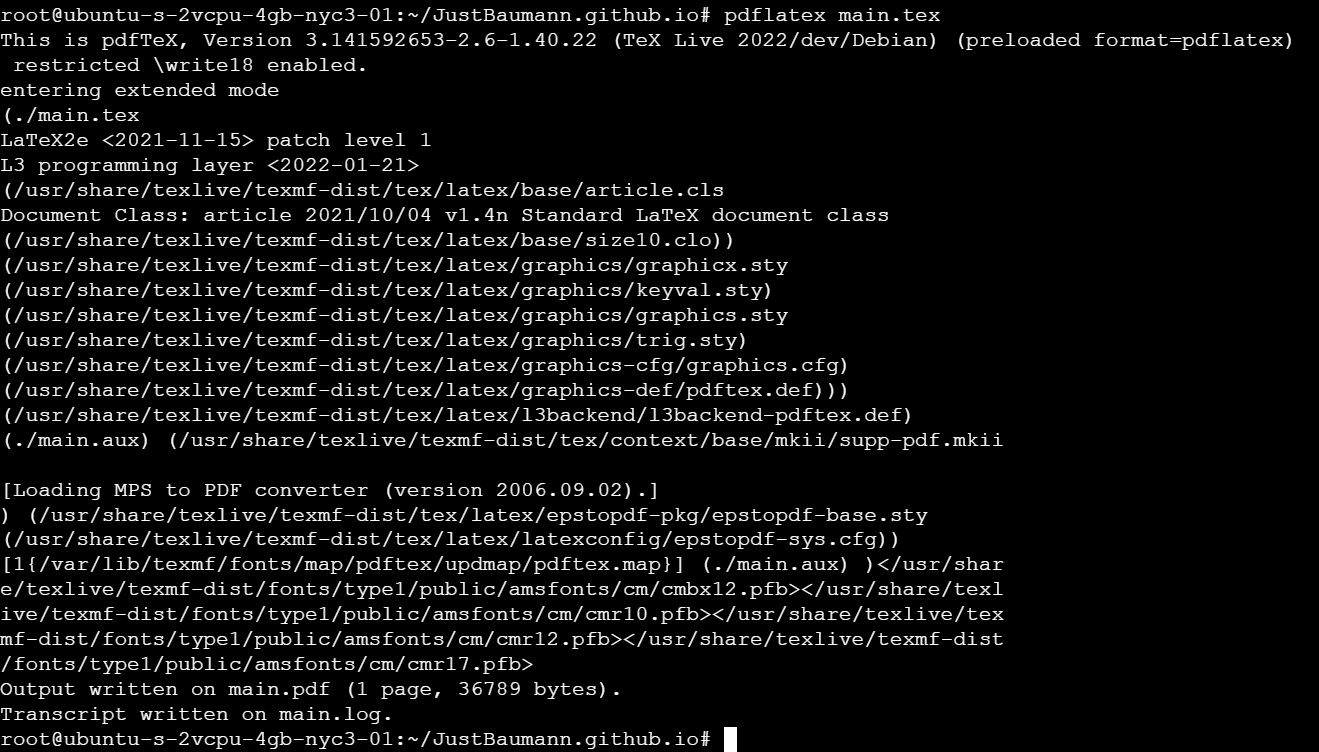
\includegraphics[width=0.5\linewidth]{png/cmdoverleaf.png}
    \caption{Cmd Output of compiled overleaf}
    \label{fig:placeholder}
\end{figure}

The output saved to main.pdf, we can commit this to github and check it out in the repository with the following commands 

\begin{minted}{bash}
    git add main.pdf 
    git commit -m "commited compiled pdf"
    git push   
\end{minted}

You can then see the compiled pdf, as evidenced here
\begin{figure}
    \centering
    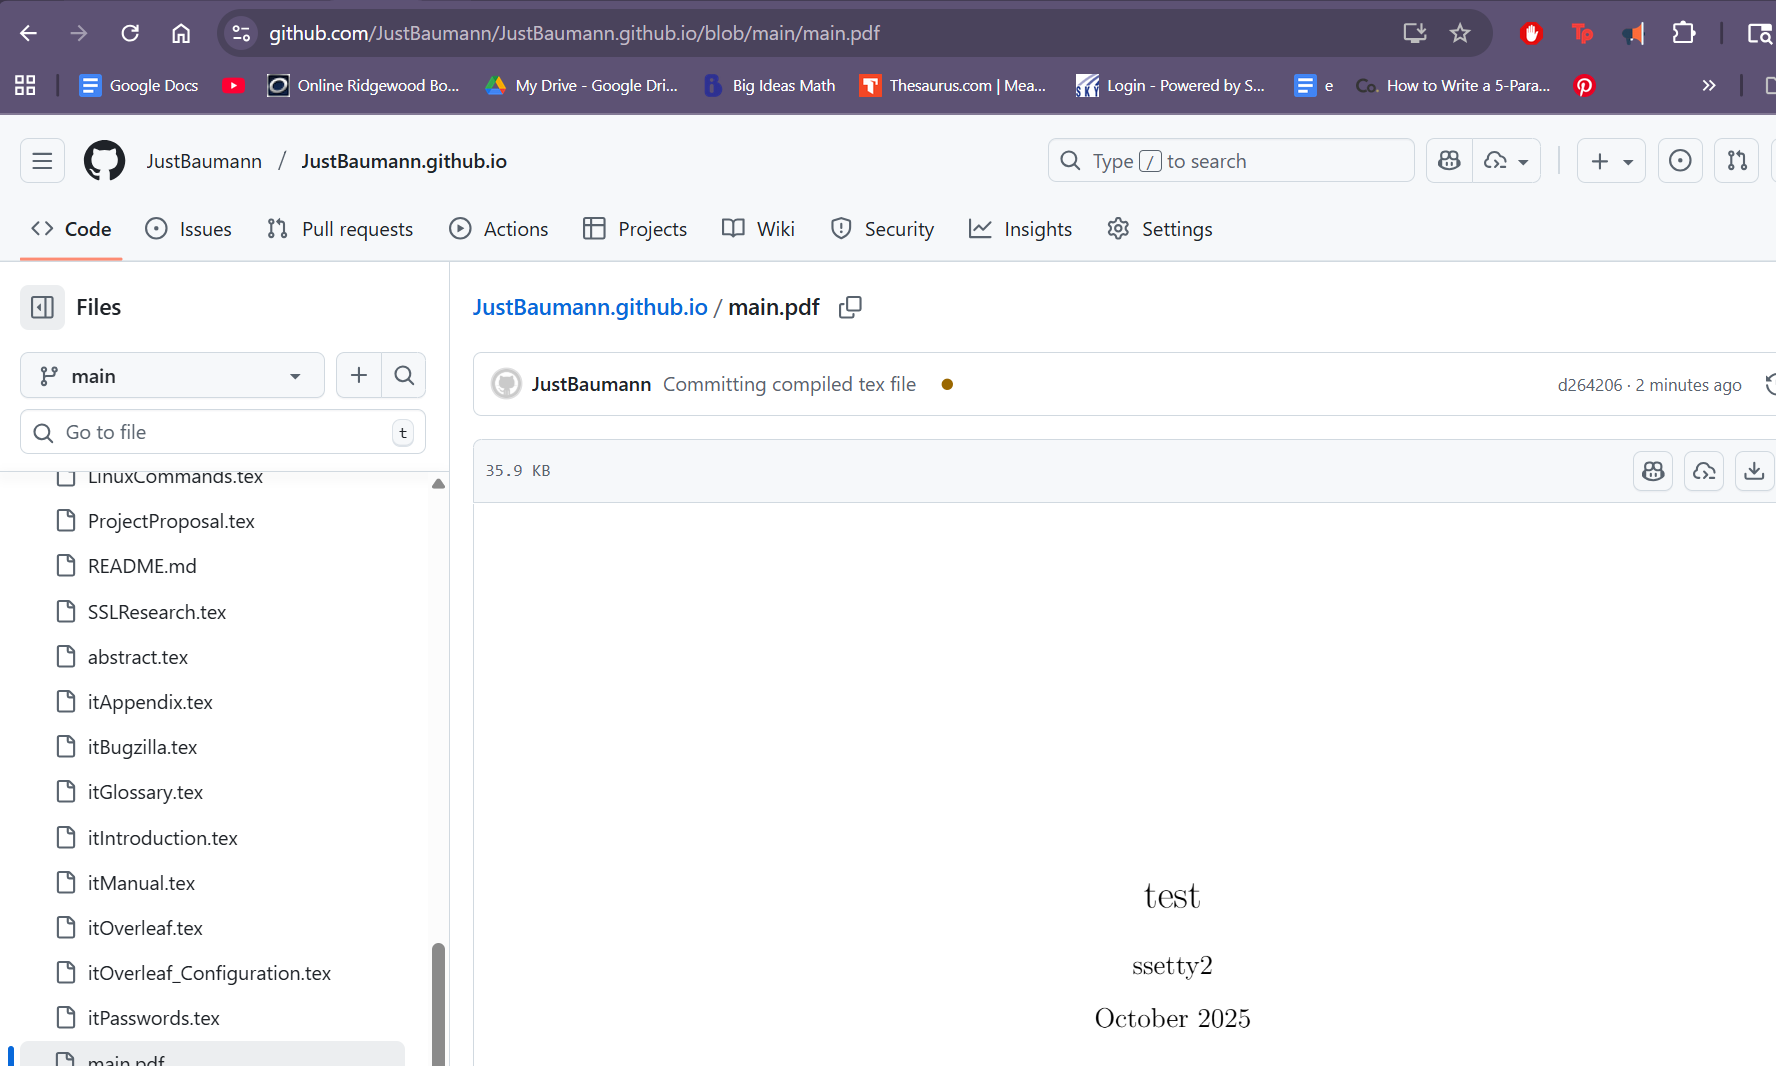
\includegraphics[width=0.5\linewidth]{png/overleafpdf.png}
    \caption{PDF Output of compiled overleaf}
    \label{fig:placeholder}
\end{figure}
